% Chapter Template

\chapter{Visualizaciones} % Main chapter title

\label{VISUALIZACIÓN} % Change X to a consecutive number; for referencing this chapter elsewhere, use \ref{ChapterX}

%----------------------------------------------------------------------------------------
%	SECTION 1
%----------------------------------------------------------------------------------------

\section{Representaciones clásicas del mutualismo}

Las visualizaciones son una herramienta cada día más importante en el análisis de la información, y en particular en la ciencia de redes. La representación gráfica resulta fundamental en el análisis exploratorio pero también para la síntesis de los resultados. Para redes ecológicas se emplean gráficos de uso común en la representación de redes sociales \cite{freeman2012social}. Quizá porque su tamaño es reducido en comparación con otras aplicaciones, no ha habido apenas desarrollo de herramientas y gráficas específicas para este campo de aplicación \cite{yoon20043d, kazanci2007econet}.

En el análisis del mutualismo se utilizan de forma reiterada dos representaciones: el diagrama bipartito y la matriz de interacción. Ambas  son sencillas y ponen de manifiesto la separación entre clases de especies, pero tienen inconvenientes importantes. 

En el diagrama bipartito se disponen las especies en dos filas paralelas, ya sean horizontales o verticales
y se unen aquellas que interactúan.

\begin{figure}[h!]
\centering
\includegraphics[scale=0.33]{Figures/VIS_bipartito_SD_001.png}
\caption{Diagrama bipartito de una red de dispersores en New Jersey \cite{baird1980selection}.}
\label{fig:VIS_bipartito_SD_001}
\end{figure}

En el ejemplo de la figura \ref{fig:VIS_bipartito_SD_001} la red es de un tamaño reducido, puede distinguirse el núcleo de plantas más conectadas (de la $1$ a la $4$ y los enlaces se ven con claridad. Cuando el número de especies supera unas pocas decenas, la situación cambia de forma radical.

\begin{figure}[h!]
\centering
\includegraphics[scale=0.4]{Figures/VIS_bipartito_SD_020.png}
\caption{Red de dispersores en Nava Correhuelas, Sierra de Cazorla, España. Compilada por Pedro Jordano, no publicada.}
\label{fig:VIS_bipartito_SD_020}
\end{figure}

La red de la figura \ref{fig:VIS_bipartito_SD_020} tiene $58$ especies y $150$ enlaces, frente a $28$ especies y $50$ enlaces de la anterior. Es una red de dimensiones moderadas, pero ya es muy complicado seguir los detalles del gráfico. A pesar de ello, algunos autores consiguen resultados excelentes con redes de dimensiones similares a las de este segundo ejemplo, jugando con formas, colores y tamaños \cite{dakos2014critical}. Cuando se llega al centenar de especies, la zona central degenera en una mancha en la que es imposible distinguir los enlaces. Por este motivo, en la literatura sobre mutualismo solo aparecen gráficos de redes pequeñas. 

La matriz de interacción ofrece una visión más rica si los nodos se ordenan de la forma adecuada. Colocando los más conectados en la parte superior izquierda, es fácil localizar el núcleo de especies generalistas. Con redes pequeñas como la del primer ejemplo, el resultado es muy satisfactorio.

\begin{figure}[h!]
\centering
\includegraphics[scale=0.4]{Figures/VIS_matrix_SD_001.png}
\caption{Matriz de interacción de una red de dispersores en New Jersey \cite{baird1980selection}. Las casillas coloreadas indican la existencia de enlace.}
\label{fig:VIS_matrix_SD_001}
\end{figure}

Por el contrario, la matriz de interacción se vuelve también muy confusa para redes grandes, como muestra la figura \ref{fig:VIS_matrix_PL_001}.

\begin{figure}[h!]
\centering
\includegraphics[scale=0.4]{Figures/VIS_matrix_PL_001.png}
\caption{Matriz de interacción de una red de polinizadores en Los Andes, Chile \cite{arroyo1982community}.}
\label{fig:VIS_matrix_PL_001}
\end{figure}


\section{Visualizaciones basadas en \textit{k-magnitudes}}

En este apartado se describen dos nuevos tipos de visualización que se basan en las \textit{k magnitudes} definidas en el capítulo anterior: el diagrama polar y el diagrama zigurat.

\subsection{El diagrama polar}

El diagrama polar se inspira en el \textit{fingerprint plot}, desarrollado por Álvarez-Hamelin \textit{et al} y que se basa en la descomposición \textit{k-core} \cite{alvarez2005k}. Los autores emplearon la técnica para reducir la información y poder visualizar redes muy grandes con índice $k$ máximo del orden de varias decenas. Los nodos se ubican de manera concénrica, a una distancia inversamente proporcional a la \textit{k-shell} a la que pertenecen. No se representan todos los enlaces, solo los más pesados. Una versión más evolucionada no utiliza los nodos sino las \textit{k-shell} que se disponen en espiral \cite{barbera2015critical}.

\begin{figure}[h!]
\centering
\includegraphics[scale=0.6]{Figures/VIS_M_PL_034_polar.png}
\caption[PolarExample]{Diagrama polar de una comunidad de polinizadores en la isla de Chiloé (Chile) \cite{smith2005diversity}.}
\label{fig:VIS_M_PL_034_polar}
\end{figure}

En nuestro caso hemos conservado la idea del diagrama concéntrico y la coloración en función del \textit{k-shell}, pero el diagrama polar difiere en todo lo demás de los dos mencionados. Para empezar, la red es bipartita. Cada clase se sitúa en un de los semiplanos y se utiliza la forma de los nodos para remarcar esta diferencia. El centro de cada especie se sitúa a una distancia $k_{radius}$ del origen de coordenadas, recordemos que el valor mínimo de esta magnitud es $1$. El ángulo se distribuye al azar por el algoritmo de representación para evitar al máximo la superposición de nodos. El área es proporcional al $k_{degree}$ y el color, propio de la \textit{k-shell}. Los enlaces no se representan.

Se puede elegir incluir los nombres de todas las especies, de ninguna, o de un pequeño número, por defecto las tres más centrales y las tres más alejadas. Adicionalmente, el usuario puede elegir que se añadan los histogramas de las tres \textit{k-magnitudes}, que contienen información muy valiosa.

La figura \ref{fig:VIS_M_PL_034_polar} es la representación polar de una red de polinizadores, que hemos elegido por ser una red mutualista tipo tanto por tamaño, anidamiento, modularidad y valores de las \textit{k magnitudes}, todos ellos no demasiado alejados de la media (tabla \ref{table:table_results}). El histograma de la distribución por \textit{k shells} tiene forma de bañera, muy repetido en estas redes. Hay unos pocos nodos domninantes y centrales, de índice $k = 5$ y un número importante de especies en las \textit{shells exteriores}. Es una red de elevada asimetría ($0.66$, véase tabla \ref{table:table_rewiring}).

La utilidad del diagrama polar se descubre al comparar varias redes, incluso si son de tamaños muy dispares. En la figura \ref{fig:VIS_Modvskdegree3}, hemos escogido tres redes situadas en ambos extremos y en el centro del diagrama \ref{fig:ESTATICA_corrfigs} (derecha). La red de polinizadores $PL\_010$  tiene un valor de $Modularity$ bajo $(0.25)$, y alto el de $\overline {k}_{degree}$ $(4.57)$. El diagrama polar muestra la estructura en capas del mutualismo. Esta es mucho más evidente en la red $SD\_007$ ($Modularity:    0.28$, $\overline {k}_{degree}: 2.34$). La distribución de $\overline {k}_{degree}$ es mucho más abrupta, con dos especies muy dominantes. La imagen transmite la idea de ser una red con mayor organización jerárquica que $PL\_010$.

La red $PL\_021$ es grande y fuertemente modular ($Modularity: 0.57$, $\overline {k}_{degree}: 1.23$). La distribución de $\overline {k}_{degree}$ es aun más abrupta. Se ha incluido en la parte inferior izquierda, la distribución de densidades que ya aparecía en la figura \ref{fig:ESTATICA_density_plots} porque la escala logarítmica en el eje horizontal permite ver mejor las diferencias.

\begin{figure}[h!]
\centering
\includegraphics[scale=0.75]{Figures/VIS_Modvskdegree3.PDF}
\caption[PolarExample]{Comparación de tres redes mediante sus diagramas polares.}
\label{fig:VIS_Modvskdegree3}
\end{figure}

A pesar de que el diagrama polar ofrece una nueva visión de las comunidades mutualistas, tiene limitaciones. Como en toda estrategia de reducción de al información hay que renunciar a representar detalles en favor de una mejor visibilidad, en este caso los enlaces. No se trata de un detalle menor, así que se ha desarrollado un segundo tipo de diagrama que los toma como base de su construcción.

\subsection{El diagrama zigurat}

El diagrana zigurat se ha creado para mostrar la estructura de \textit{k shells} de una red bipartita y todos los enlaces entre sus nodos. La idea básica consiste en agrupar las especies en \textit{shells} que se representan como pequeños zigurats(\footnote{Según el DRAE: Torre escalonada y piramidal, característica de la arquitectura religiosa asiria y caldea.}). Las dos \textit{shells} máximas se colocan en el eje de simetría horizontal, ligeramente hacia la izquierda. El resto, se distribuyen siguiendo una disposición en forma de almendra, que deja un gran espacio libre para dibujar los enlaces.

\begin{figure}[h!]
\centering
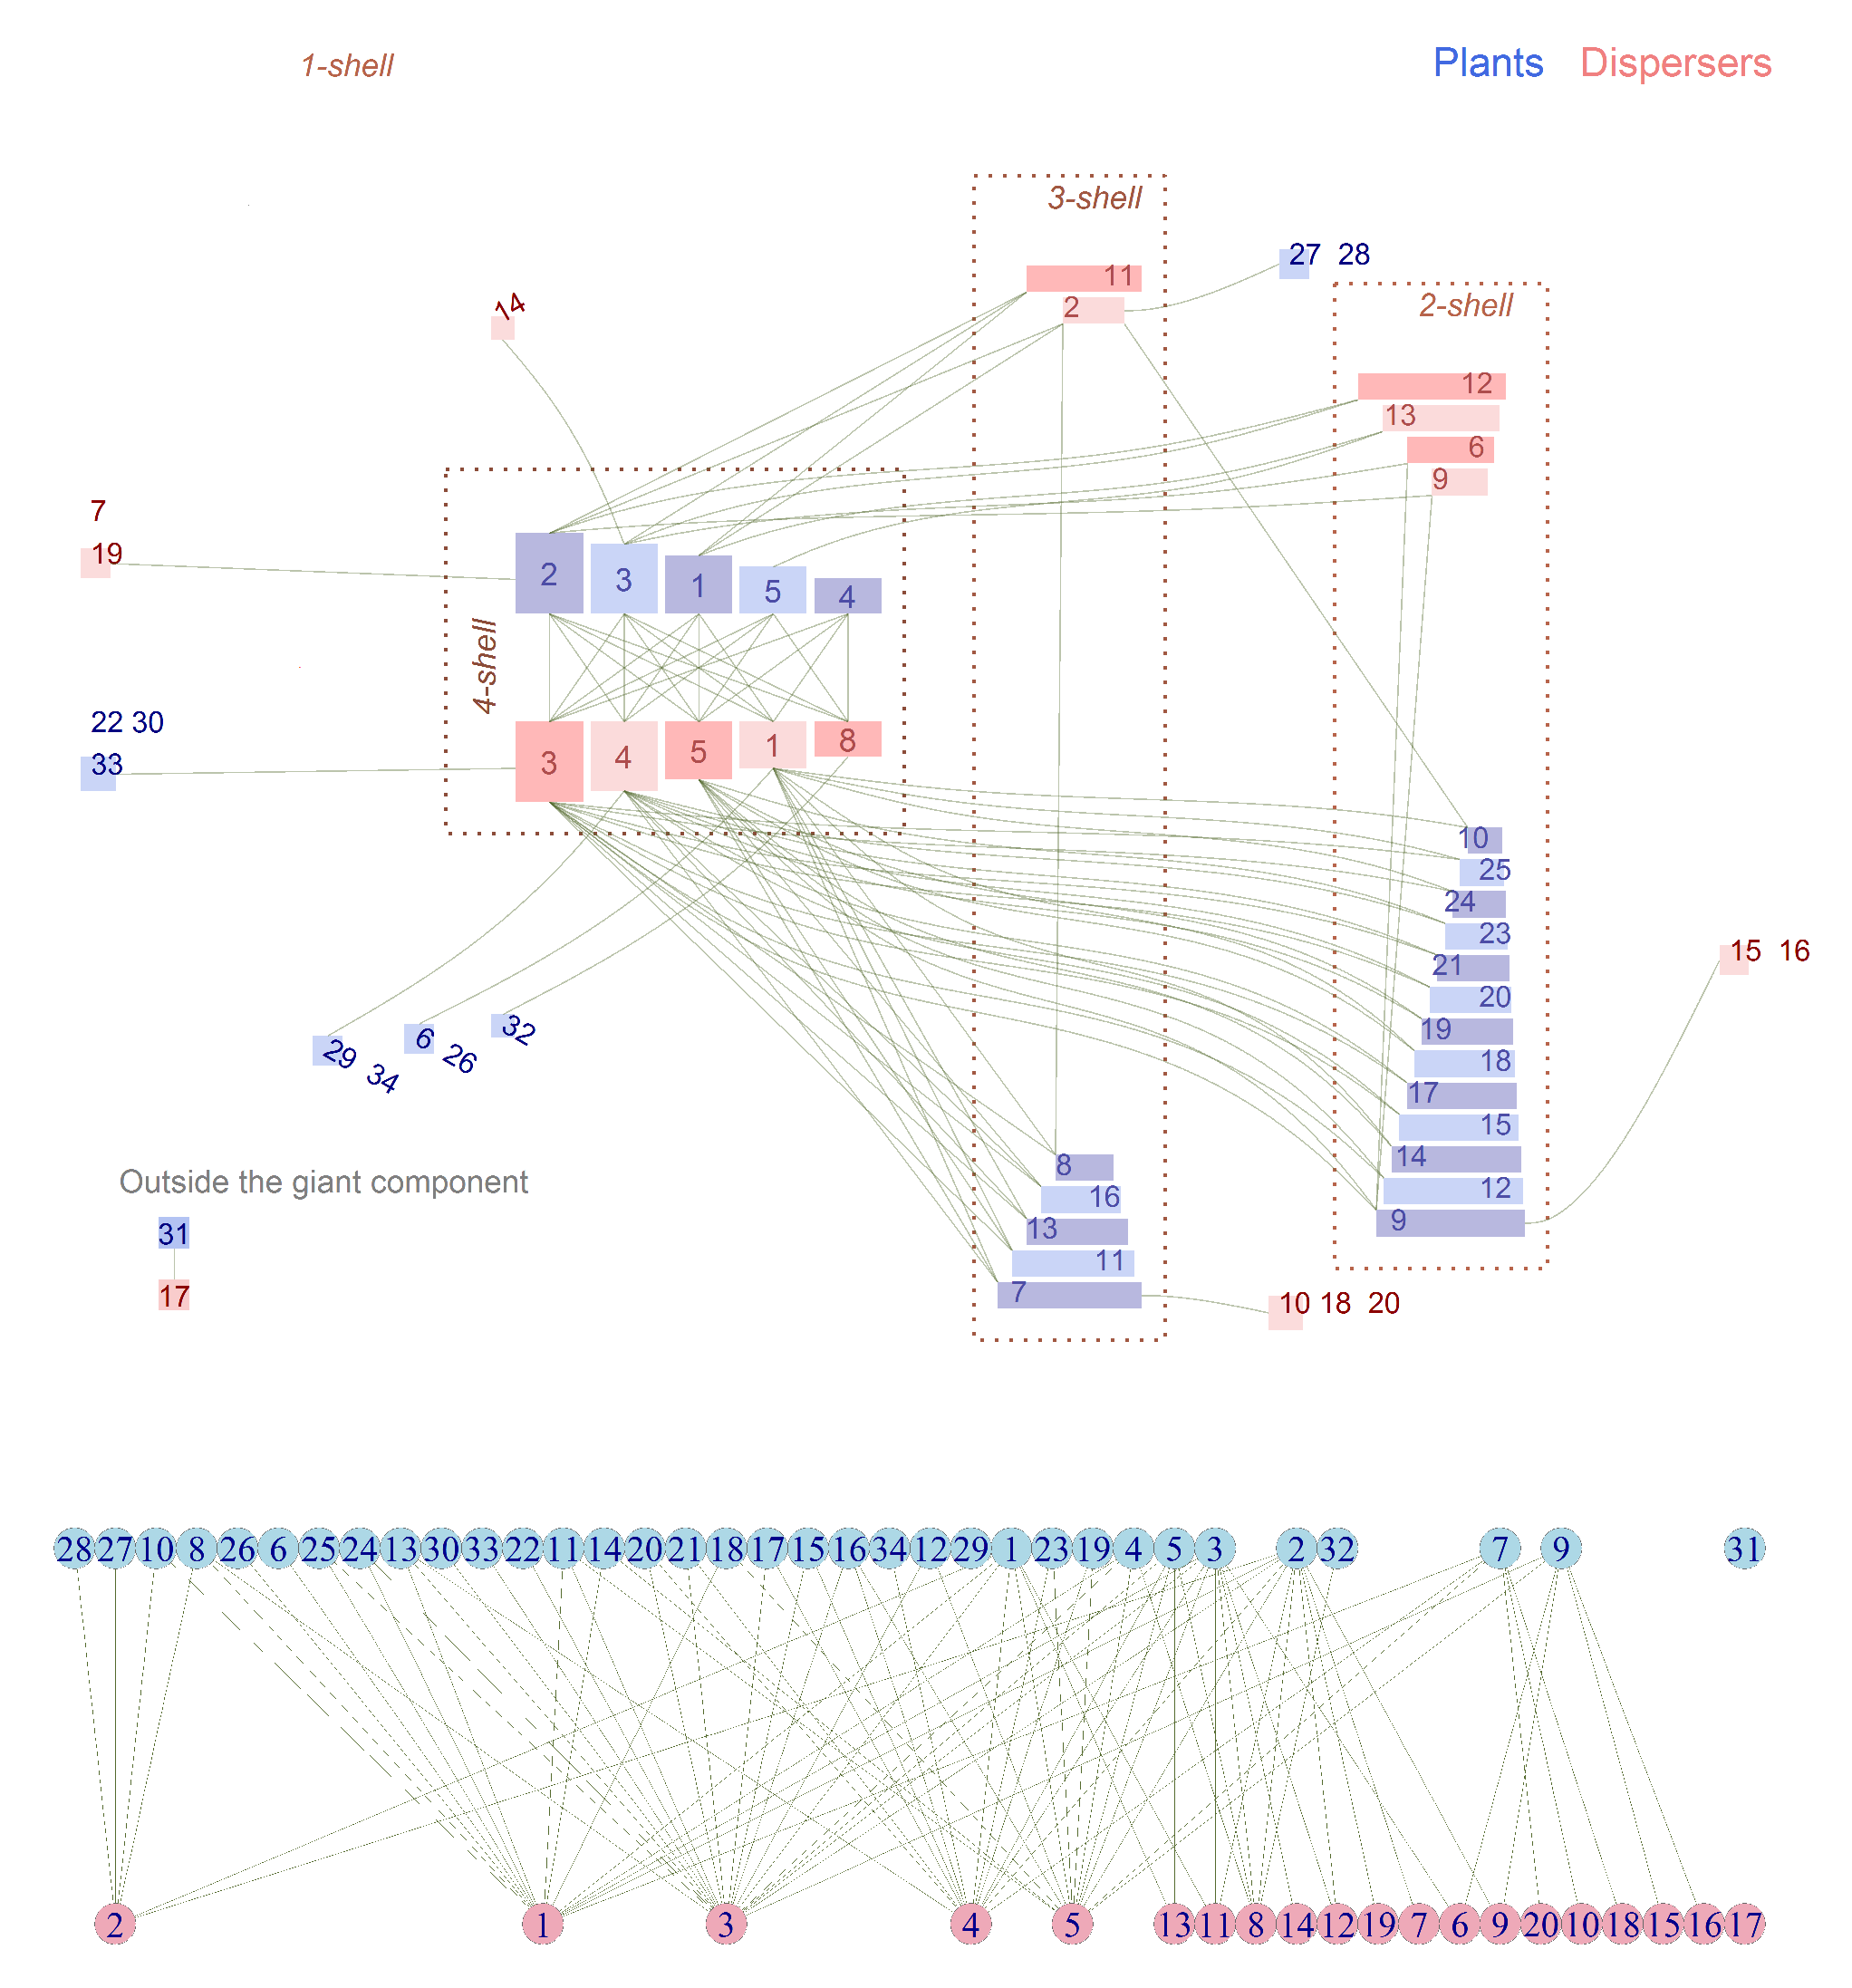
\includegraphics[scale=0.4]{Figures/VIS_ALL_SD_004.eps}
\caption {Diagrama zigurat de una comunidad de aves frugívoras de Puerto Rico, con $54$ especies y $95$ enlaces \cite{carlo2003avian}. Abajo el diagrama bipartito.}
\label{fig:ziggurat}
\end{figure}

En la \textit{shell} máxima las especies se ordenan por $k_{degree}$, con el valor mayor a la izquierda. En el resto, se ordenan por $k_{radius}$, correspondiendo la base del zigurat a la especie de menor $k_{radius}$.

Las especies de la \textit{1-shell} se disponen como una nube el torno a la almendra central. Si, como sucede a menudo, varias especies de esta \textit{shell} comparten enlace, se dibujan de forma agrupada y con un único enlace.

En algunas redes, los autores han incluido observaciones de especies que no están conectadas con la componente gigante. En ese caso, se representa el fragmento inconexo, pero no se tiene en cuenta para la \textit{k descomposición}.

Por último, es importante recalcar que en el diagrama zigurat, las áreas no transmiten información sobre tamaños de la población.

La red de la figura \ref{fig:ziggurat} es de pequeño tamaño. En el gráfico bipartito todavía se pueden seguir los enlaces individuales. Sin embargo, el zigurat ofrece una visión mucho más rica de la organización con cuatro \textit{shells} internas y una pequeña \textit{1-shell}. Se pueden descubrir con facilidad algunos patrones, como la baja conectividad entre especies de las \textit{shells} de menor índice $k$, o la relativa importancia de la especie dispersora $2$ que en el bipartito aparece en el extremo izquierdo.

\begin{figure}[ht!]
\centering
\includegraphics[scale=0.16]{Figures/VIS_zig_pl_024.png}
\caption {Plant Pollinator network number 024, Mosquin, T., and J. E. H. Martin (1967). Observations on the pollination biology of plants on Melville Island, N.W.T., Canada. \textit{Canadian Field Naturalist} 81:201-205.}
\label{fig:ziggurat}
\end{figure}


\clearpage
\begin{figure}[ht!]
\centering
\includegraphics[scale=0.22]{Figures/VIS_M_PL_031_ziggurat.png}
\caption {Plant Pollinator network number 031}
\label{fig:ziggurat}
\end{figure}

\clearpage
\begin{figure}[ht!]
\centering
\includegraphics[scale=0.6]{Figures/VIS_M_PL_010_ziggurat.png}
\caption {Red de polinizadores $M\_PL\_010$ (Elberling \& Olesen, no publicada), con $107$ especies y $456$ enlaces. Su diagrama polar puede verse en la figura \ref{fig:VIS_Modvskdegree3}.}
\label{fig:ziggurat}
\end{figure}

\clearpage
\section{Resultados}

Nunc posuere quam at lectus tristique eu ultrices augue venenatis. Vestibulum ante ipsum primis in faucibus orci luctus et ultrices posuere cubilia Curae; Aliquam erat volutpat. Vivamus sodales tortor eget quam adipiscing in vulputate ante ullamcorper. Sed eros ante, lacinia et sollicitudin et, aliquam sit amet augue. In hac habitasse platea dictumst.


\section{Conclusiones}

Nunc posuere quam at lectus tristique eu ultrices augue venenatis. Vestibulum ante ipsum primis in faucibus orci luctus et ultrices posuere cubilia Curae; Aliquam erat volutpat. Vivamus sodales tortor eget quam adipiscing in vulputate ante ullamcorper. Sed eros ante, lacinia et sollicitudin et, aliquam sit amet augue. In hac habitasse platea dictumst.
